% ==============================================================================
% CAPÍTULO 7: SITIO WEB DE LA EMPRESA (Orquestador del Capítulo)
% ==============================================================================
\preportadacapitulo{7}{Sitio Web de la Empresa}

\newpage
\section{Capítulo 7: Sitio Web de la Empresa}\label{cap:sitio_web}

% [INSTRUCCIÓN]: Sitio web de la empresa desarrolladora. Contenido propio de esta versión.
% [VERIFICAR]: el sitio publicado muestra un correo de ejemplo; reemplazarlo por leonel.barriosmay@gmail.com y volver a tomar la captura de la sección de contacto.

El sitio web es la presentación pública de NEXWARE: da a conocer a la empresa, describe lo que ofrece y permite que un posible cliente la contacte. Este capítulo define su contenido, su planificación y el diseño de sus pantallas. Además de ser la vitrina de la empresa, el sitio sirve de punto de entrada a los sistemas que desarrolla, entre ellos el Sistema de Gestión de Postulación y Asistencia del Comedor Universitario.

\subsection{7.1. Sitio Web Corporativo}

\subsubsection{7.1.1. Información principal}

El sitio presenta a NEXWARE con la información que ya define el Capítulo~\hyperref[cap:sqap]{2}:

\begin{itemize}
    \item \textbf{Quiénes somos:} empresa de desarrollo de sitios web y aplicaciones móviles a medida, de Santa Cruz de la Sierra, formada por dos socios.
    \item \textbf{Misión:} diseñar y desarrollar sitios web y aplicaciones móviles a medida, sin plantillas, de modo que cada línea de código responda al problema concreto del cliente, con calidad verificable mediante pruebas automatizadas y control de versiones (sección 2.4).
    \item \textbf{Visión:} ser una empresa de desarrollo de software de referencia en Santa Cruz de la Sierra, reconocida por convertir las ideas de sus clientes en soluciones confiables, mantenibles y adaptadas a su realidad (sección 2.5).
    \item \textbf{Eslogan:} «Si no existe, lo programamos.», con la frase de apoyo «Tu idea, plasmada.» (sección 2.7).
\end{itemize}

\subsubsection{7.1.2. Planificación}

El sitio se diseña como una página de una sola columna con secciones que se recorren de arriba abajo, y se construye como sitio estático con Astro y TypeScript, probado con Vitest, en español y en inglés (Capítulo~\hyperref[cap:paps]{1}). La planificación se organiza en tres pasos:

\begin{enumerate}
    \item \textbf{Contenido:} se redactan los textos de cada sección (identidad, servicios, proceso de trabajo y contacto) con la información de este capítulo.
    \item \textbf{Prototipo:} se dibujan las pantallas descritas en la sección 7.1.4 antes de programarlas, para validar el recorrido del visitante.
    \item \textbf{Publicación:} se programa el sitio, se prueba en computadora y en celular y se publica (sección 7.2).
\end{enumerate}

\subsubsection{7.1.3. Planificación de comunicación con los clientes}

\paragraph{7.1.3.1. Información de la empresa.}

La información de la empresa se muestra en la vista de inicio (nombre, eslogan y descripción) y en la sección «Nosotros» (los dos socios). La misión y la visión se definen en el Capítulo~\hyperref[cap:sqap]{2}; el sitio publicado no las muestra como tarjetas. Esta información responde a la primera pregunta del visitante: quién es NEXWARE y por qué confiar en ella.

\paragraph{7.1.3.2. Descripción de productos y servicios.}

Se presentan los servicios de NEXWARE (desarrollo de sitios web a medida y de aplicaciones móviles) y el producto realizado como caso de estudio: el sistema de gestión de postulación y asistencia del comedor universitario, con una breve descripción de lo que resuelve. Los servicios y sus precios se definen en el Capítulo~\hyperref[cap:mercado]{8}.

\paragraph{7.1.3.3. Formulario de contacto.}

El visitante deja su nombre, un correo de contacto y un mensaje que describe lo que necesita. El formulario valida los campos antes de enviarlos y notifica por correo al equipo de NEXWARE. El cliente recibe una confirmación de recepción y se le responde en el plazo que la empresa fije.

\paragraph{7.1.3.4. Diseño responsivo.}

El sitio se adapta al ancho de la pantalla. En celular las secciones se apilan en una columna, el menú pasa a un botón desplegable y los botones tienen un tamaño cómodo para el dedo. En computadora las tarjetas y las cuadrículas se distribuyen en varias columnas. Así el sitio se puede leer sin esfuerzo desde un teléfono o desde una computadora.

\subsubsection{7.1.4. Diseño y prototipo}

Se describen las ocho zonas de la página de inicio del sitio publicado, en el orden en que las ve el visitante. Las capturas son del sitio en línea (sección 7.2).

\paragraph{7.1.4.1. Vista de inicio.}

Es la primera pantalla. El encabezado muestra el logotipo, un menú con anclas a cada sección (Servicios, Stack, Proceso, Portafolio, Nosotros y Contacto), el selector de idioma español/inglés, un botón para cambiar entre modo claro y oscuro y el botón «Hablemos», que lleva al formulario de contacto. Debajo aparecen la etiqueta «Web · Móvil · A medida — Santa Cruz, Bolivia», el eslogan «Si no existe, lo programamos.» como título principal, la frase «Tu idea, plasmada.», una descripción breve y dos botones: «Cuéntanos tu idea» y «Ver proyecto demo». A la derecha, una cuadrícula de cuadros que recuerda al logotipo de píxeles.

\begin{figure}[H]
\caption{Vista de inicio del sitio web de NEXWARE}
\label{fig:sitio_inicio}
\centering
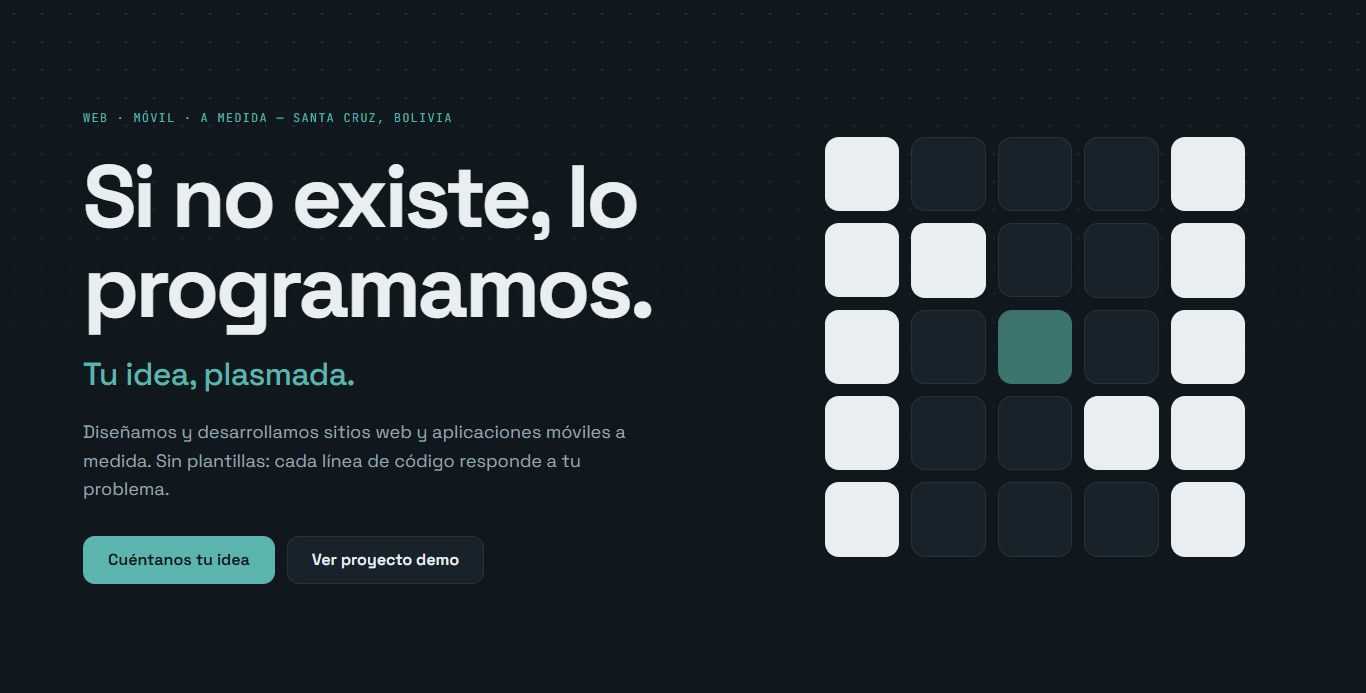
\includegraphics[width=\textwidth]{images/169_Sitio_NEXWARE_Inicio.png}

\smallskip
\noindent\raggedright\textit{Nota.} Elaboración propia. Captura del sitio publicado, 19 de noviembre de 2026.
\end{figure}

\paragraph{7.1.4.2. Servicios.}

Tres tarjetas presentan lo que ofrece NEXWARE: web a medida (sitios y aplicaciones con React y TypeScript), aplicaciones móviles (una sola base de código para Android e iOS con Flutter) y \textit{backend} e inteligencia artificial (APIs con Spring Boot y servicios de IA con FastAPI).

\begin{figure}[H]
\caption{Sección de servicios del sitio web de NEXWARE}
\label{fig:sitio_servicios}
\centering
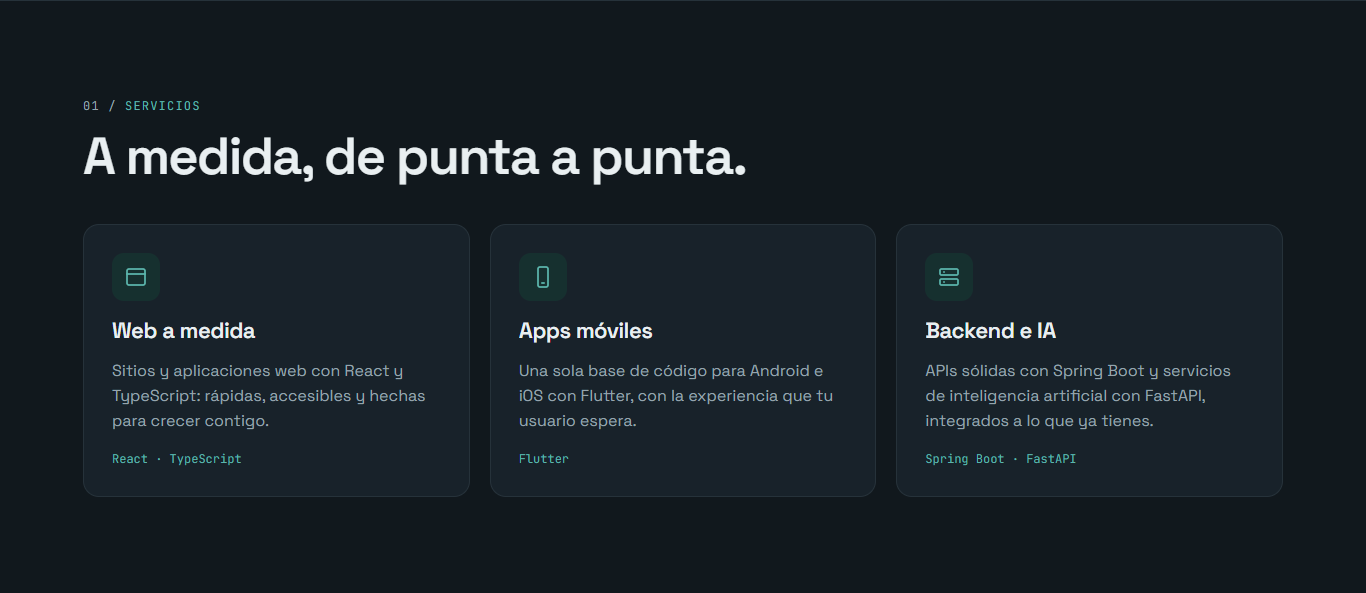
\includegraphics[width=\textwidth]{images/158_Sitio_NEXWARE_Servicios.png}

\smallskip
\noindent\raggedright\textit{Nota.} Elaboración propia. Captura del sitio publicado, 19 de noviembre de 2026.
\end{figure}

\paragraph{7.1.4.3. Stack tecnológico.}

Cuatro tarjetas explican las tecnologías de la empresa y por qué se eligieron: React con TypeScript para la interfaz, Spring Boot para el \textit{backend}, Flutter para el móvil y FastAPI para la inteligencia artificial. Cada tarjeta lleva el área, el nombre de la tecnología y una línea de justificación.

\begin{figure}[H]
\caption{Sección de stack tecnológico del sitio web de NEXWARE}
\label{fig:sitio_stack}
\centering
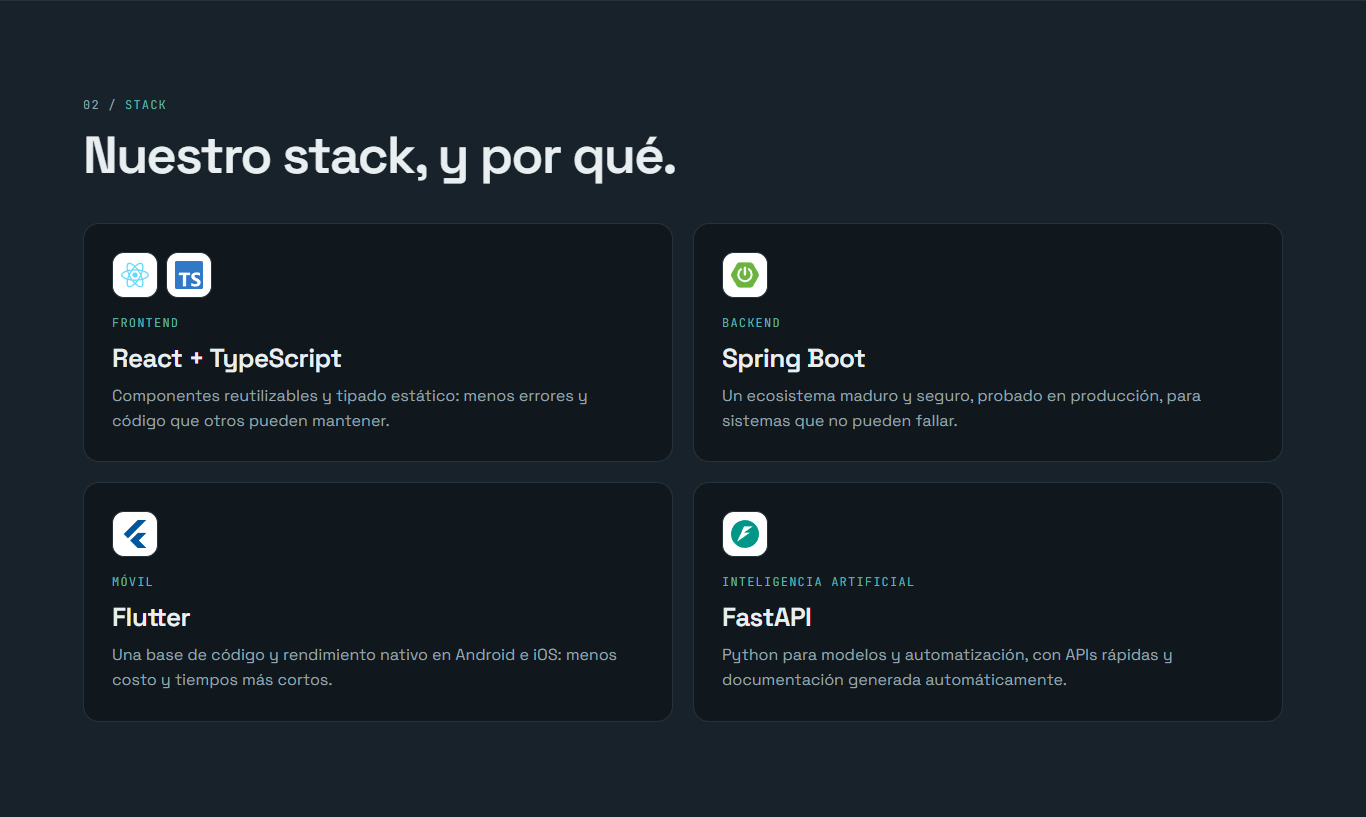
\includegraphics[width=\textwidth]{images/159_Sitio_NEXWARE_Stack.png}

\smallskip
\noindent\raggedright\textit{Nota.} Elaboración propia. Captura del sitio publicado, 19 de noviembre de 2026.
\end{figure}

\paragraph{7.1.4.4. Proceso de trabajo.}

Una secuencia de cuatro pasos numerados muestra cómo trabaja NEXWARE con un cliente: descubrimiento (entender el problema y definir el alcance), diseño (prototipar las pantallas y el flujo), desarrollo (ciclos cortos con entregas frecuentes) y entrega (despliegue, documentación y acompañamiento). Es la versión visible para el cliente del proceso unificado del Capítulo~\hyperref[cap:procesos_puds]{3}.

\begin{figure}[H]
\caption{Sección de proceso de trabajo del sitio web de NEXWARE}
\label{fig:sitio_proceso}
\centering
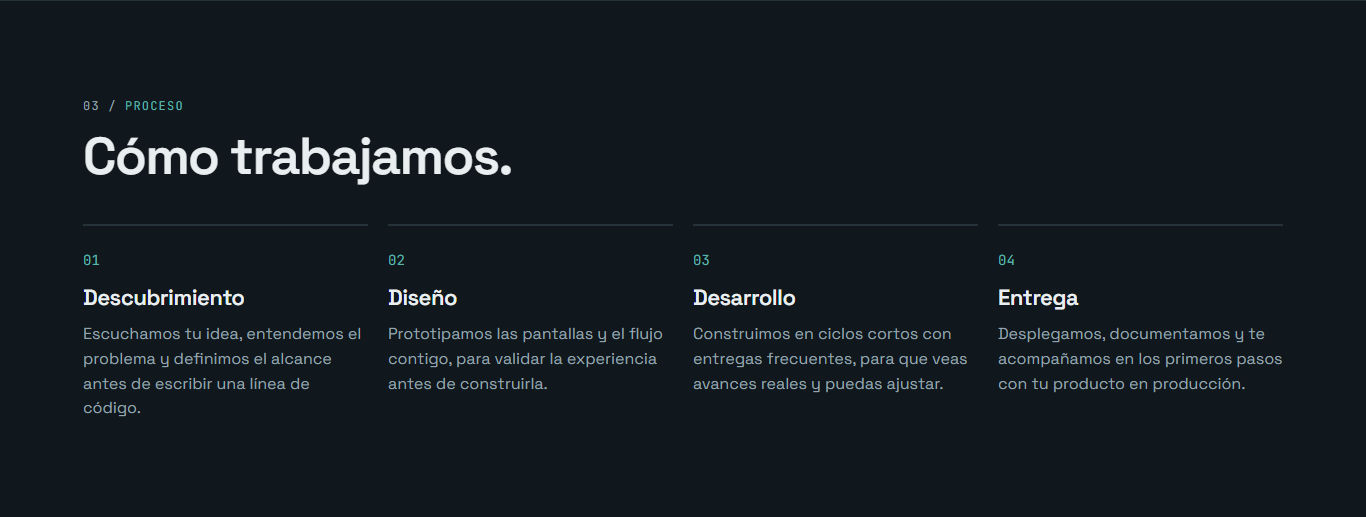
\includegraphics[width=\textwidth]{images/160_Sitio_NEXWARE_Proceso.png}

\smallskip
\noindent\raggedright\textit{Nota.} Elaboración propia. Captura del sitio publicado, 19 de noviembre de 2026.
\end{figure}

\paragraph{7.1.4.5. Portafolio.}

Presenta el proyecto demo de la empresa, ComedorUAGRM: una captura del panel, la descripción de lo que resuelve, las tecnologías usadas (Spring Boot, React, Flutter y FastAPI) y el botón «Ver demo», que lleva al sistema en funcionamiento. Es el acceso del sitio a los sistemas que NEXWARE desarrolla (sección 7.1.3.2).

\begin{figure}[H]
\caption{Sección de portafolio del sitio web de NEXWARE}
\label{fig:sitio_portafolio}
\centering
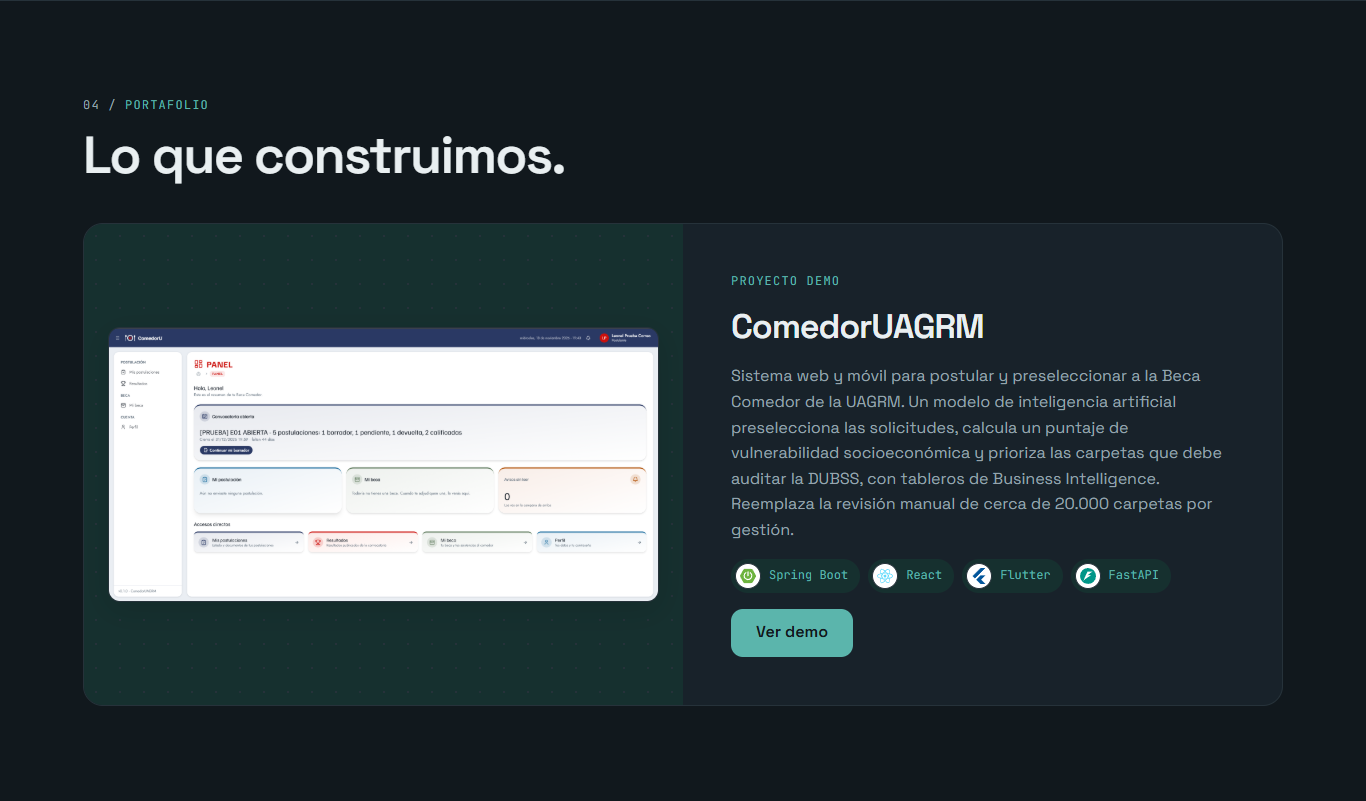
\includegraphics[width=\textwidth]{images/161_Sitio_NEXWARE_Portafolio.png}

\smallskip
\noindent\raggedright\textit{Nota.} Elaboración propia. Captura del sitio publicado, 19 de noviembre de 2026.
\end{figure}

\paragraph{7.1.4.6. Nosotros.}

Presenta a los dos socios, Mauro Boris Gutierrez Primintela y Carlos Leonel Barrios Mayorga, ambos con el cargo de CEO y desarrollador \textit{full stack}, cada uno con un enlace «Ver CV». Incluye también la explicación del nombre («Nexo + software») y del logotipo hecho de píxeles, que representa cada pieza encajando en su lugar.

\begin{figure}[H]
\caption{Sección «Nosotros» del sitio web de NEXWARE}
\label{fig:sitio_nosotros}
\centering
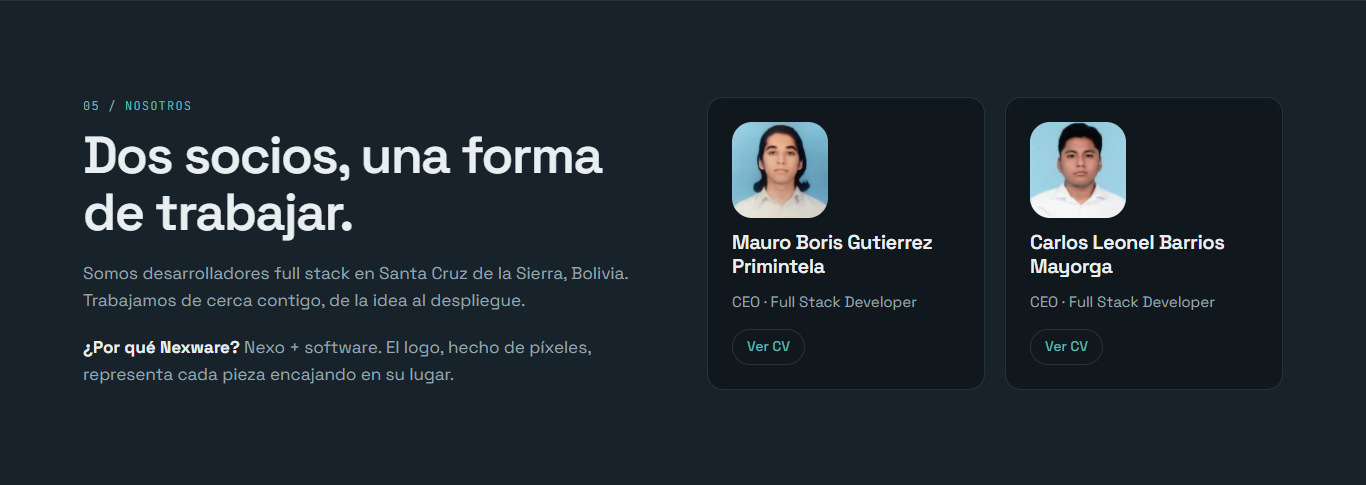
\includegraphics[width=\textwidth]{images/162_Sitio_NEXWARE_Nosotros.png}

\smallskip
\noindent\raggedright\textit{Nota.} Elaboración propia. Captura del sitio publicado, 19 de noviembre de 2026.
\end{figure}

\paragraph{7.1.4.7. Contacto.}

Muestra el correo de contacto de la empresa y un formulario con los campos nombre, correo y «¿Qué quieres construir?», con el botón «Enviar mensaje». Incluye un campo oculto contra envíos automáticos. El correo de contacto de NEXWARE es \texttt{leonel.barriosmay@gmail.com}; el sitio publicado muestra por ahora un correo de ejemplo (\texttt{ceo.desarrollo@nexware.example}) que debe reemplazarse por ese.

\begin{figure}[H]
\caption{Sección de contacto del sitio web de NEXWARE}
\label{fig:sitio_contacto}
\centering
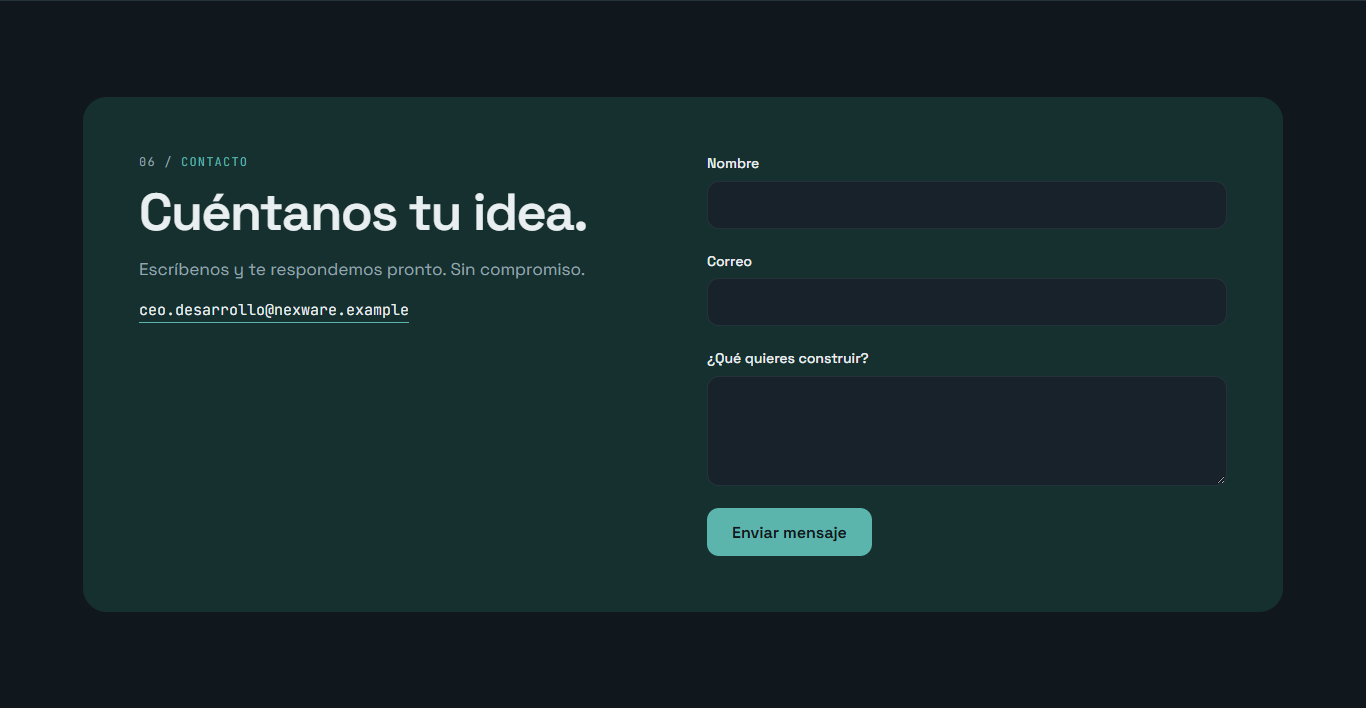
\includegraphics[width=\textwidth]{images/163_Sitio_NEXWARE_Contacto.png}

\smallskip
\noindent\raggedright\textit{Nota.} Elaboración propia. Captura del sitio publicado, 19 de noviembre de 2026.
\end{figure}

\paragraph{7.1.4.8. Pie de página.}

Repite el nombre y el eslogan de la empresa, los enlaces a las secciones del sitio y los enlaces legales (términos y condiciones, política de privacidad, política de cookies y aviso legal), y el aviso de derechos reservados de 2026. El aviso aclara que se trata de un proyecto académico ficticio de Ingeniería de Software 2.

\begin{figure}[H]
\caption{Pie de página del sitio web de NEXWARE}
\label{fig:sitio_pie}
\centering
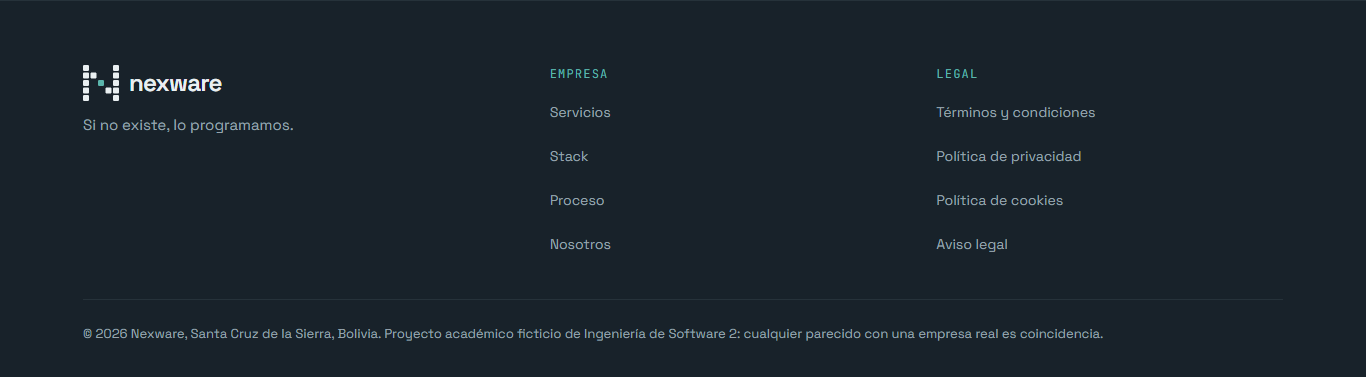
\includegraphics[width=\textwidth]{images/164_Sitio_NEXWARE_Pie.png}

\smallskip
\noindent\raggedright\textit{Nota.} Elaboración propia. Captura del sitio publicado, 19 de noviembre de 2026.
\end{figure}

\paragraph{7.1.4.9. Muro de comentarios (previsto).}

El sitio publicado no incluye un muro de comentarios de clientes. Cuando NEXWARE tenga clientes con comentarios publicables, una sección mostraría su opinión; mientras tanto no se publican testimonios que no existan.

\subsection{7.2. Acceso al Sitio Web}

\subsubsection{7.2.1. URL}

El sitio web de NEXWARE está publicado en \url{https://d38nteg7p7v4qz.cloudfront.net/landing-page/es/} (versión en español; el sitio también tiene versión en inglés).

\subsubsection{7.2.2. QR}

La Figura~\ref{fig:qr_nexware} contiene el código QR que lleva al sitio desde un teléfono móvil.

\begin{figure}[H]
\caption{Código QR del sitio web de NEXWARE}
\label{fig:qr_nexware}
\centering

\includegraphics[width=4cm]{images/168_QR_Sitio_NEXWARE.png}

\smallskip
\noindent\raggedright\textit{Nota.} Elaboración propia. Dirige a la versión en español del sitio.
\end{figure}
